%%%%%%%%%%%%%%%%%%%%%%%%%%%%%%%%%%%%%%%%%
% Short Sectioned Assignment LaTeX Template Version 1.0 (5/5/12)
% This template has been downloaded from: http://www.LaTeXTemplates.com
% Original author:  Frits Wenneker (http://www.howtotex.com)
% License: CC BY-NC-SA 3.0 (http://creativecommons.org/licenses/by-nc-sa/3.0/)
%%%%%%%%%%%%%%%%%%%%%%%%%%%%%%%%%%%%%%%%%

%----------------------------------------------------------------------------------------
%	PACKAGES AND OTHER DOCUMENT CONFIGURATIONS
%----------------------------------------------------------------------------------------

\documentclass[paper=a4, fontsize=11pt]{scrartcl} % A4 paper and 11pt font size

% ---- Entrada y salida de texto -----

\usepackage[T1]{fontenc} % Use 8-bit encoding that has 256 glyphs
\usepackage[utf8]{inputenc}
%\usepackage{fourier} % Use the Adobe Utopia font for the document - comment this line to return to the LaTeX default

% ---- Idioma --------

\usepackage[spanish, es-tabla]{babel} % Selecciona el español para palabras introducidas automáticamente, p.ej. "septiembre" en la fecha y especifica que se use la palabra Tabla en vez de Cuadro

% ---- Otros paquetes ----

\usepackage{url} % ,href} %para incluir URLs e hipervínculos dentro del texto (aunque hay que instalar href)
\usepackage{amsmath,amsfonts,amsthm} % Math packages
%\usepackage{graphics,graphicx, floatrow} %para incluir imágenes y notas en las imágenes
\usepackage{graphics,graphicx, float, subfig} %para incluir imágenes y colocarlas

% Para hacer tablas comlejas
%\usepackage{multirow}
%\usepackage{threeparttable}

%\usepackage{sectsty} % Allows customizing section commands
%\allsectionsfont{\centering \normalfont\scshape} % Make all sections centered, the default font and small caps

\usepackage{fancyhdr} % Custom headers and footers
\pagestyle{fancyplain} % Makes all pages in the document conform to the custom headers and footers
\usepackage{eurosym} % Para poder añadir el símbolo del euro
\fancyhead{} % No page header - if you want one, create it in the same way as the footers below
\fancyfoot[L]{} % Empty left footer
\fancyfoot[C]{} % Empty center footer
\fancyfoot[R]{\thepage} % Page numbering for right footer
\renewcommand{\headrulewidth}{0pt} % Remove header underlines
\renewcommand{\footrulewidth}{0pt} % Remove footer underlines
\setlength{\headheight}{13.6pt} % Customize the height of the header

\numberwithin{equation}{section} % Number equations within sections (i.e. 1.1, 1.2, 2.1, 2.2 instead of 1, 2, 3, 4)
\numberwithin{figure}{section} % Number figures within sections (i.e. 1.1, 1.2, 2.1, 2.2 instead of 1, 2, 3, 4)
\numberwithin{table}{section} % Number tables within sections (i.e. 1.1, 1.2, 2.1, 2.2 instead of 1, 2, 3, 4)

\setlength\parindent{0pt} % Removes all indentation from paragraphs - comment this line for an assignment with lots of text

\newcommand{\horrule}[1]{\rule{\linewidth}{#1}} % Create horizontal rule command with 1 argument of height

\usepackage{listings}
\usepackage{dsfont}
\usepackage{booktabs}
%----------------------------------------------------------------------------------------
%	TÍTULO Y DATOS DEL ALUMNO
%----------------------------------------------------------------------------------------

\title{	
\normalfont \normalsize 
\textsc{\textbf{Taller de Geometría y Topología} \\ Grado en Matemáticas \\ Universidad de Granada} \\ [25pt] % Your university, school and/or department name(s)
\horrule{0.5pt} \\[0.4cm] % Thin top horizontal rule
\huge Ejercicios del Grupo 3  \\
	Grafos, Polígonos y Poliedros % The assignment title
\horrule{2pt} \\[0.5cm] % Thick bottom horizontal rule
}
\author{	
		Elena Tudela Castro \\
		Raimundo Morales Solier \\
		Simón López Vico \\
		Francisco Gallego Salido \\
		Alberto Jesús Durán López} % Nombre y apellidos
\date{\normalsize\today} % Incluye la fecha actual

%----------------------------------------------------------------------------------------
% DOCUMENTO
%----------------------------------------------------------------------------------------

\begin{document}

\maketitle % Muestra el Título

\newpage %inserta un salto de página

%\tableofcontents % para generar el índice de contenidos

% \listoffigures

% \listoftables




\section{Grafos y Poliedros}


\subsection{Actividades I.1}

\begin{enumerate}
	\item Coger varios triángulos equiláteros y pegarlos unos con otros hasta conseguir un poliedro.
	
	Los poliedros que se pueden obtener uniendo varios triángulos equiláteros pegados son: tetraedro, octaedro e icosaedro.
	
	\item Une tres triángulos equiláteros a un punto y completa la figura con otro.
	
	Se obtiene un tetraedro.
	
	\item Construye un poliedro que tenga 4 triángulos equiláteros en todos sus vértices. Lo mismo con cinco triángulos. ¿Es posible con 6 o más?
	
	Con 4 triángulos equiláteros por vértice se obtiene un octaedro y, con 5, un icosaedro.
	
	No sería posible una construcción de 6 o más triángulos equiláteros por vértice ya que estamos trabajando con figuras geométricas cuyo ángulo interno sea menor que 2$\pi$. Con seis triángulos el ángulo interno sería 2$\pi$ y tendríamos un plano, y con más de seis estaríamos en un espacio hiperbólico.
	
	\item Un poliedro regular es aquel cuyas caras son polígonos regulares congruentes y con el mismo número de polígonos en cada vértice. Uniendo polígonos de 3,4,5,6,7... lados construye todos los poliedros regulares posibles. ¿Cómo los llamarías? ¿Cuándo vale V-A+C?
	
	Veamos respecto a cada caso:
	
	\begin{itemize}
		\item Con 3: tetraedro, octaedro e icosaedro.
		\item Con 4: cubo.
		\item Con 5: dodecaedro.
	\end{itemize}
	
	A partir de 6 no se podría por lo comentado en el ejercicio anterior.
	
	En todos ellos se cumple $V-A+C=2$
	
\end{enumerate}

\subsection{Actividades I.2}
\begin{enumerate}
	\item ¿Cuál es la suma de los ángulos de un polígono de n lados en el plano?
	
	La suma de los ángulos es $(n-1)\cdot \pi$.
	
	\item Determina el ángulo total de defecto de los 5 poliedros regulares y de los construidos en la actividad anterior.
	
	
	\begin{table}[H]
		\centering
		\begin{tabular}{@{}cccc@{}}
			\toprule
			\textbf{Polígono} & \textbf{Nº vértices} & \textbf{Ángulo de defecto por vértice} & \textbf{Ángulo de defecto total} \\ \midrule
			Tetraedro         & 4                    & $\pi$                                      & 4$\pi$                           \\
			Octaedro          & 6                    & 2$\pi$/3                                   & 4$\pi$                           \\
			Cubo              & 8                    & $\pi$/2                                    & 4$\pi$                           \\
			Icosaedro         & 12                   & $\pi$/3                                    & 4$\pi$                           \\
			Dodecaedro        & 20                   & $\pi$/5                                    & 4$\pi$                           \\ \bottomrule
		\end{tabular}
	\end{table}
	
	Haciendo los cálculos obtenemos que el ángulo total de defecto para todos ellos es $4\pi$, tanto en regulares como no regulares
	
\end{enumerate}

\subsection{Actividad I.3}
\begin{enumerate}
	\item Discute con otros compañeros una posible demostración de la fórmula de Descartes.
	
	Para empezar, denotemos los siguientes términos:
	
	\begin{itemize}
		\item Ángulo de defecto de un vértice $i$: $T_i=2\pi-S_i$, donde $S_i=$ \{Suma de los ángulos, dentro de las caras, que se unen en el vértice $i$\}.
		
		\item Angulo total de defecto, $T=$ \{Suma de los ángulos de defecto en todos los vértices del poliedro\} $=4\pi$.
	\end{itemize}
	
	Sea $S$ la suma total de todos los ángulos de todas las caras del poliedro y $V$ el número de vértices; se tendrá entonces que:
	
	\[
	S = \sum_{i=1}^{V}S_i = \sum_{i=1}^{V} (2\pi-T_i)=2\pi V -\sum_{i=1}^{V}S_i = 2\pi V - T
	\]
	
	Por otro lado, consideramos las caras de nuestro poliedro. En cada cara hay $n$ aristas, y se cumple que la suma de los ángulos de dicha cara es $\pi(n-2)$, como ya hemos visto anteriormente.
	
	Denotando $C_n$ al número de caras que tienen $n$ aristas (con $n$ desde 3 hasta un $k$) y, sabiendo que $\sum_{n=3}^{k}n\dot C_n = 2A$ ($A=$aristas, ya que cada arista pertenece a dos caras y por ello se cuenta 2 veces), se cumplirá que:
	
	\[
	S=\sum_{n=3}^{k}(n-2)\pi C_n=(\sum_{n=3}^{k} nC_n-2\sum_{n=3}^{k}C_n)\pi = (2A-2C)\pi 
	\]
	
	Por tanto, utilizando todo lo anterior y despejando:
	
	\begin{align*}
		2\pi V - T =  (2A-2C)\pi
		\Longrightarrow T  = 2 \pi V-(2A-2C)\pi
		\Longrightarrow T = 2\pi(C-A+V)  
	\end{align*}
	
	Pero como sabemos que $T=4\pi$, finalmente obtenemos:
	\[
	2=C-A+V
	\]
\end{enumerate}

\subsection{Actividades I.4}
\begin{enumerate}
	\item El ángulo de defecto de un poliedro convexo puede calcularse rotando el poliedro en un círculo alrededor de su vértice. Explica cómo.
	
	Ponemos una cara del poliedro sobre un papel y marcamos una de las aristas que sale del vértice que hemos elegido. Rotamos el poliedro manteniendo la arista marcada sobre el papel. Repetimos el proceso hasta que la primera arista que hemos utilizado vuelva a tocar el papel, y marcamos la arista. El ángulo entre las dos aristas señaladas será el ángulo de defecto del vértice.
	
	\item Si rotamos el poliedro a lo largo de una curva cerrada en la superficie del mismo que no pase por los vértices, ¿qué ángulo de defecto podemos medir y cómo?
	
	Distingamos varias posibilidades:
	
	\begin{itemize}
		\item Si la curva no rodea ningún vértice no podemos medir ningún ángulo.
		\item Si la curva cerrada rodea un único vértice (que es lo mismo que rodear $n-1$ vértices en un poliedro de $n$ vértices) estamos en el caso del ejercicio anterior.
		\item Si la curva engloba todos los vértices, tendremos el ángulo de defecto total, $T$.
		\item Si la curva engloba $k$ vértices, tendremos $2\Pi-($\textit{Suma de los ángulos, dentro de las caras, que se unen en cada vértice} $k_i)$. En caso de que el poliedro sea regular, podremos obtener el ángulo de defecto de un vértice dividiendo entre $k$.
	\end{itemize}
	
	El método para medirlo sería igual que en el ejercicio anterior, rotando por las aristas donde pasa la curva.
\end{enumerate}

\subsection{Actividades Imaginación}

\begin{enumerate}
	\item Leer tu nombre al revés.
	
	Nombres de los integrantes del grupo al revés:
	\begin{itemize}
		\item Odnumiar.
		\item Nomis.
		\item Anele.
		\item Otrebla.
		\item Ocsicnarf.
	\end{itemize}
	
	\item Divide en tres partes iguales los lados de un triángulo equilátero y recorta las esquinas que resultan. ¿Qué figura queda? 
	
	Quedará un hexágono.
	
	\item Pon dos cuadrados superpuestos y rota uno de 45 grados. ¿Cuál es la intersección de los dos?
	
	Si lo rotamos tomando como punto de rotación el centro del cuadrado, obtendremos un octógono.
	
	\item Divide en tres partes iguales los lados de un cuadrado y recorta las esquinas. ¿Qué figura queda?
	
	De nuevo, obtenemos un octógono.
	
	\item ¿Cuántas aristas tiene un cubo?
	
	Tiene doce aristas.
	
	\item En la silueta que determinan las aristas de un cubo, traza un arco cerrado que pase una vez y solo una por cada vértice.
	
	\begin{figure}[H]
		\centering
		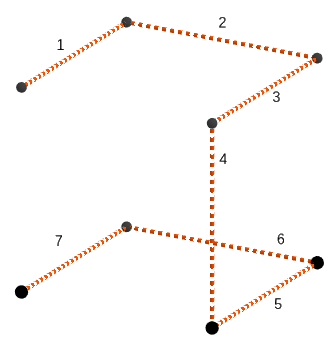
\includegraphics[scale=0.5]{images/grafos_poligonos_poliedros/a2.png}
	\end{figure}
	
	\item En una tabla de puntos 3x4 del plano, conéctalos vertical y horizontalmente. ¿Cuántos cuadrados se determinan?
	
	Se determinan seis cuadrados pequeños y otros dos formados por la unión de cuatro de los pequeños.
	
	\begin{figure}[H]
		\centering
		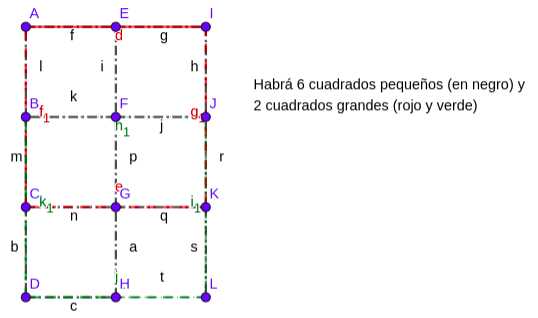
\includegraphics[scale=0.5]{images/grafos_poligonos_poliedros/a1.png}
	\end{figure}
	
	
	\item Encuentra un arco cerrado a lo largo de las aristas de la tabla anterior que pase por cada vértice uno y sólo una vez. ¿Puede hacerse lo mismo con una tabla 3x3?
	
	Utilizando la tabla anterior podremos encontrar dicho arco, pero no podrá encontrarse para una tabla 3x3.
	
	\begin{figure}[H]
		\centering
		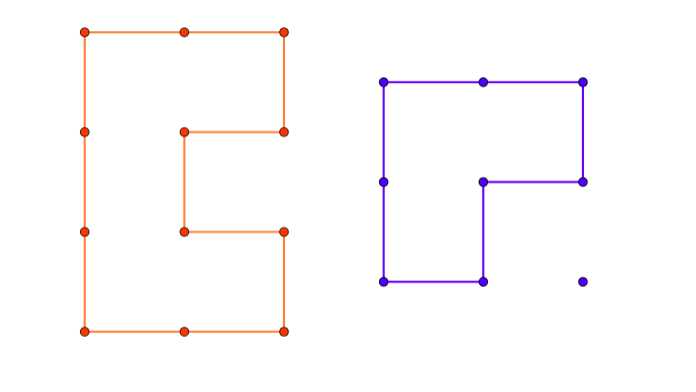
\includegraphics[scale=0.5]{images/grafos_poligonos_poliedros/a1_1.png}
	\end{figure}
	
	
	\item ¿Cuántos colores son necesarios para colorear las caras de un cubo?
	
	Con 3 colores distintos para que dos caras que comparten aristas no tengan el mismo color.
	
	\item ¿Cuál es el número de caras, vértices y aristas de un tetraedro? ¿Y de un octaedro?
	
	Tetraedro: 4 caras, 6 aristas y 4 vértices.
	
	Octaedro: 8 caras, 12 aristas y  6 vértices.
	
	\item Descansa un tetraedro sobre una cara y córtalo por la mitad. ¿Qué forma tiene la sección? Haz lo mismo con un octaedro.
	
	La figura resultante es un triángulo para el tetraedro y un hexágono para el octaedro.
	
	
	\begin{figure}[H]
		\centering
		\subfloat[]{
			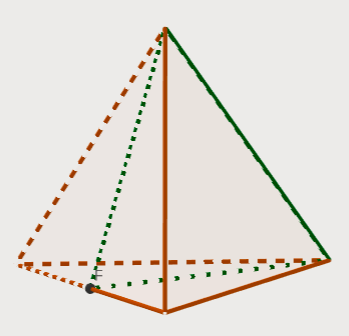
\includegraphics[scale=0.3]{images/grafos_poligonos_poliedros/a3.png}
			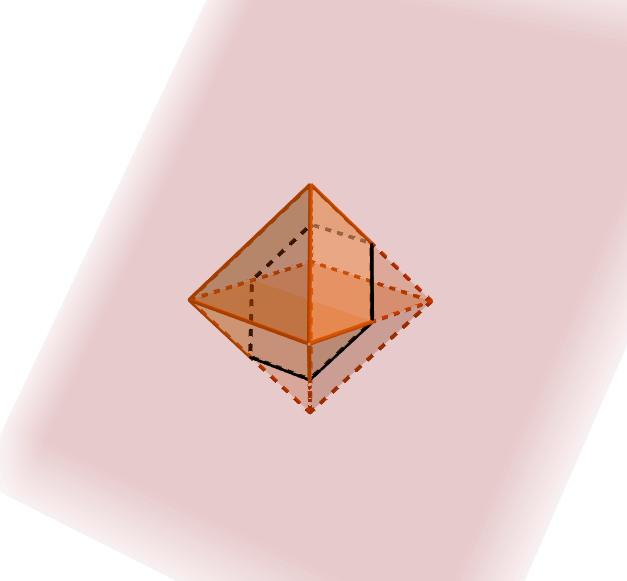
\includegraphics[scale=0.2]{images/grafos_poligonos_poliedros/a3_1.png}
		}
	\end{figure}
	
	
	\item Corta las esquinas de un triángulo equilátero hasta los puntos medios de sus lados. ¿Qué figura queda?
	
	La figura resultante es un triángulo equilátero rotado.
	
	\item Descansa en equilibrio un tetraedro sobre una arista y corta horizontalmente por la mitad. ¿Qué forma tiene la sección? Haz lo mismo con un octaedro.
	
	La figura resultante es un cuadrado en ambos casos.
	
	\begin{figure}[H]
		\centering
		\subfloat[]{
			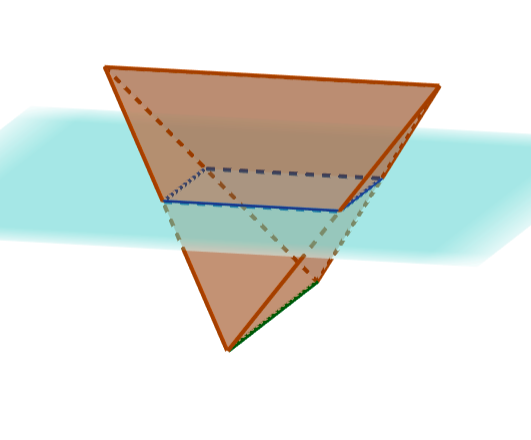
\includegraphics[scale=0.25]{images/grafos_poligonos_poliedros/a4_1.png}
			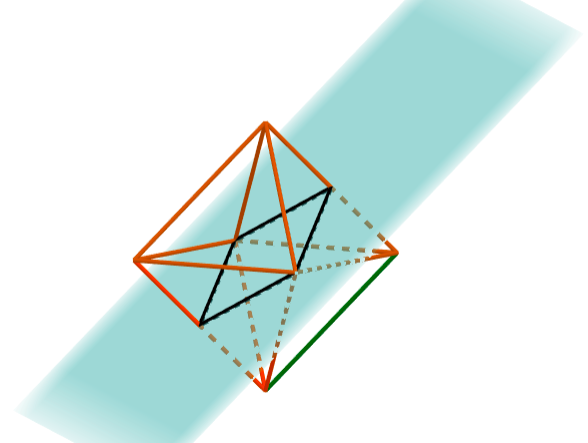
\includegraphics[scale=0.25]{images/grafos_poligonos_poliedros/a4.png}
		}
	\end{figure}
	
	
	\item Corta las esquinas de un tetraedro hasta los puntos medios de sus lados. ¿Qué figura queda?
	
	Un octaedro.
	
	\begin{figure}[H]
		\centering
		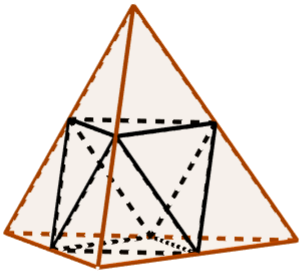
\includegraphics[scale=0.3]{images/grafos_poligonos_poliedros/a5.png}
	\end{figure}
	
	\item Si miras la silueta de un cubo desde uno de los vértices, ¿Qué silueta ves?
	
	La silueta de un hexágono.
	
	\item ¿Cuántos colores necesitamos para colorear un octaedro?
	
	Nos basta con dos colores para colorear el octaedro.
	
	\item Corta horizontalmente por la mitad un octaedro apoyado en equilibrio sobre un vértice. ¿Qué forma tiene la sección?
	
	Como vimos en el ejercicio 13, la sección tiene forma de cuadrado.
	
	\item En una tabla de puntos 3x3x3 en el espacio, únelos a lo largo, ancho y alto. ¿Puedes encontrar un camino cerrado que pase por todos los vértices menos uno, una y sólo una vez? ¿Y por todos?
	
	Como vemos en la siguiente imagen, podemos encontrar un camino cerrado que pase por todos menos 1.
	
	\begin{figure}[H]
		\centering
		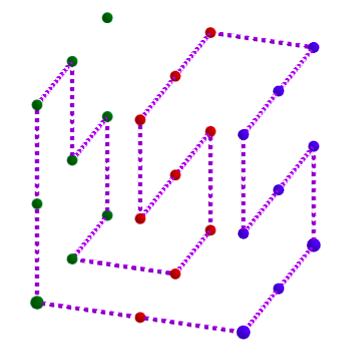
\includegraphics[scale=0.4]{images/grafos_poligonos_poliedros/a6.png}
	\end{figure}
	
	Por otra parte, no podemos hacerlo con todos los puntos porque no podemos encontrar un camino cerrado hamiltoniano que pase por todos los vértices.
	
	\item Lo mismo que el anterior con una tabla de 4x4x4 puntos.
	
	En este caso, no podremos hacerlo con todos los puntos menos 1 pero sí podremos encontrar un camino cerrado que pase por todos los puntos
	
	\begin{figure}[H]
		\centering
		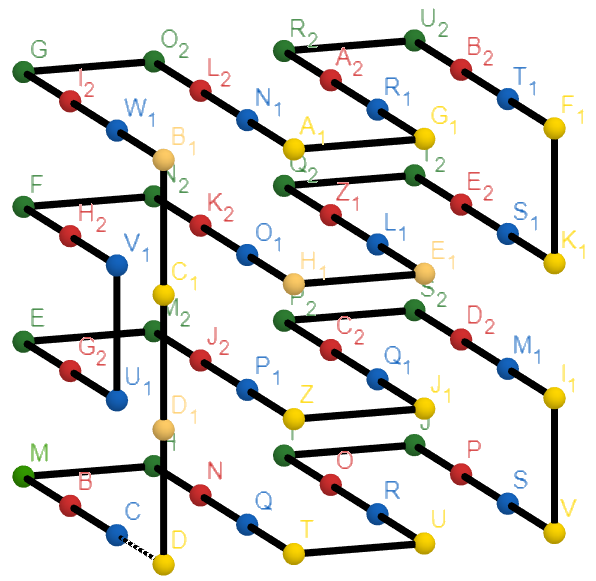
\includegraphics[scale=0.3]{images/grafos_poligonos_poliedros/ejercicio_19.png}
	\end{figure}
	
	\item Imagina un arco a través de las aristas de un octaedro que pase por todos los vértices una y sólo una vez.
	
	Lo dibujamos en Geogebra y obtenemos lo siguiente:
	
	\begin{figure}[H]
		\centering
		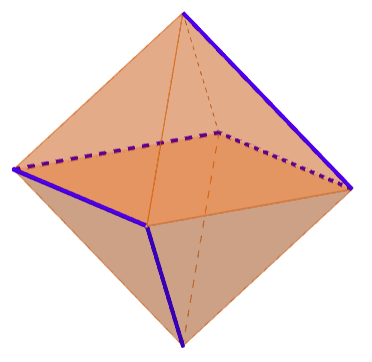
\includegraphics[scale=0.35]{images/grafos_poligonos_poliedros/arco_tetraedro.png}
	\end{figure}
	
\end{enumerate}

\section{Polígonos}

\begin{enumerate}
	\item Prueba que la suma de los ángulos interiores de un polígono de $n$ vértices es $(n-2)\pi$.
	
	Toda triangulación de un polígono de $n$ vértices tiene $n-2$ triángulos, y como la suma de los ángulos de un triángulo es $\pi$, tendremos que la suma total de los ángulos interiores es $(n-2)\pi$.
	
	\item Prueba que el ángulo total de rotación alrededor del borde de un polígono es $2\pi$.
	
	Tenemos en cuenta el apartado anterior, es decir, $\sum_{i=1}^{n} \text{ÁnguloInterior}_i = (n-2) \pi $ 
	
	\[
	\textbf{Ángulo total de rotación} = \sum_{i=1}^{n} (\pi - \text{ÁnguloInterior}_i) = n \pi - (n-2)\pi = 2\pi 
	\]
	
	\item Encuentra diferentes triangulaciones de los polígonos de la figura.
	
	\begin{figure}[H]
		\centering
		\subfloat[]{
			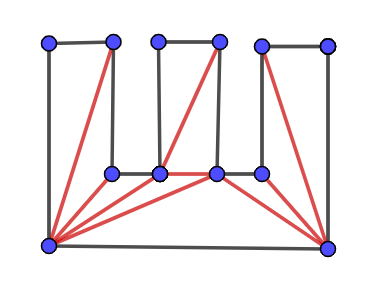
\includegraphics[scale=0.6]{images/grafos_poligonos_poliedros/triang_a_1.png}
			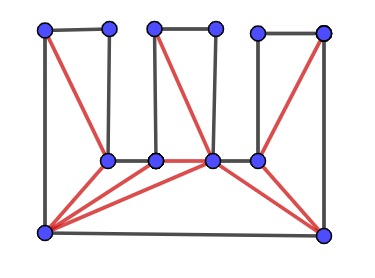
\includegraphics[scale=0.6]{images/grafos_poligonos_poliedros/triang_a_2.png}
		}
	\end{figure}
	
	
	\begin{figure}[H]
		\centering
		\subfloat[]{
			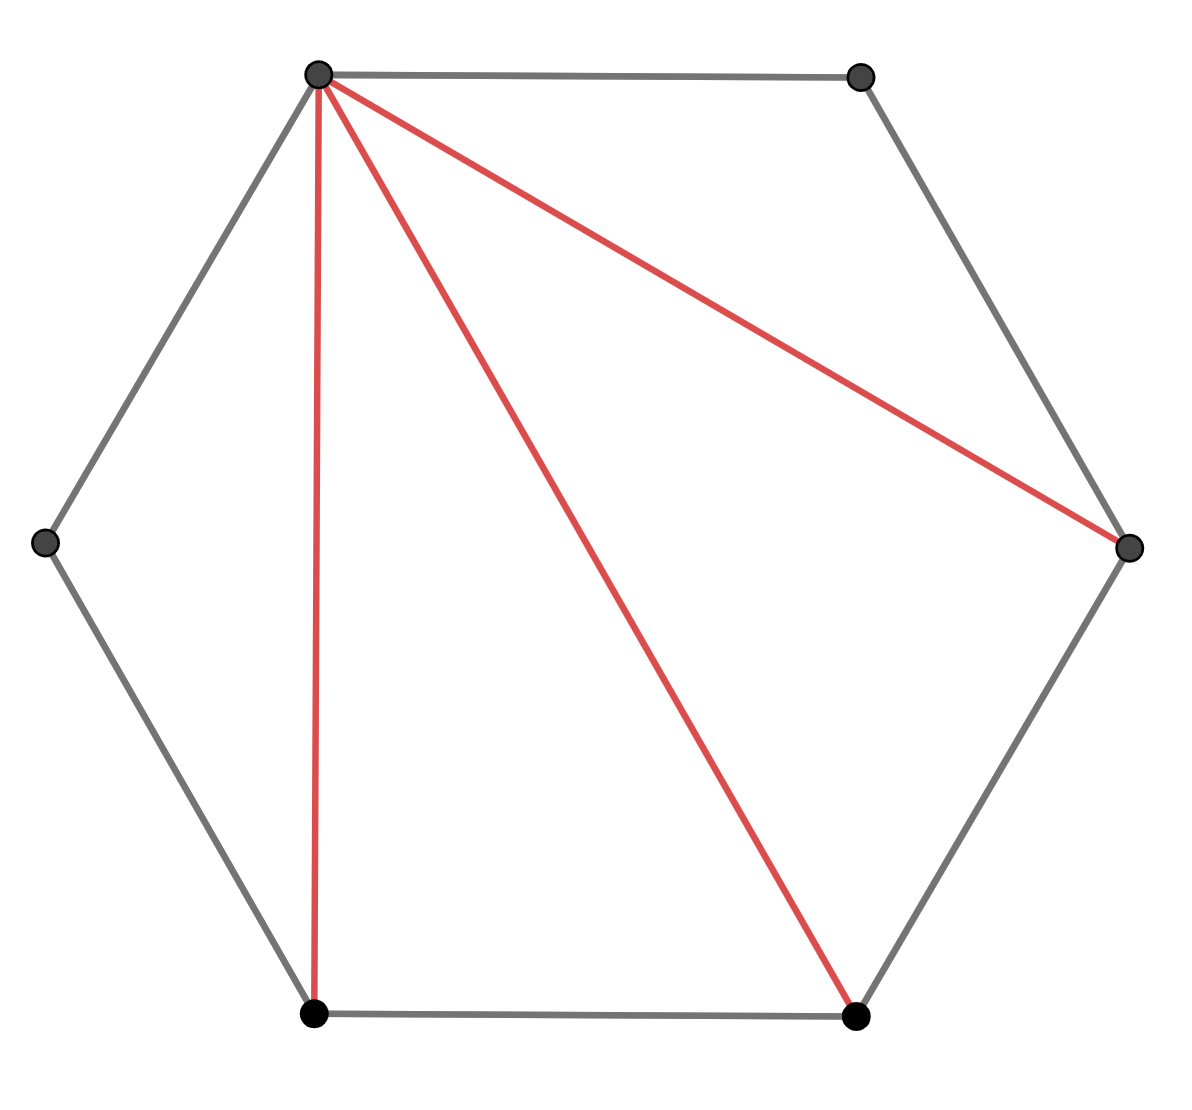
\includegraphics[scale=0.1]{images/grafos_poligonos_poliedros/triang_b_1.png}
			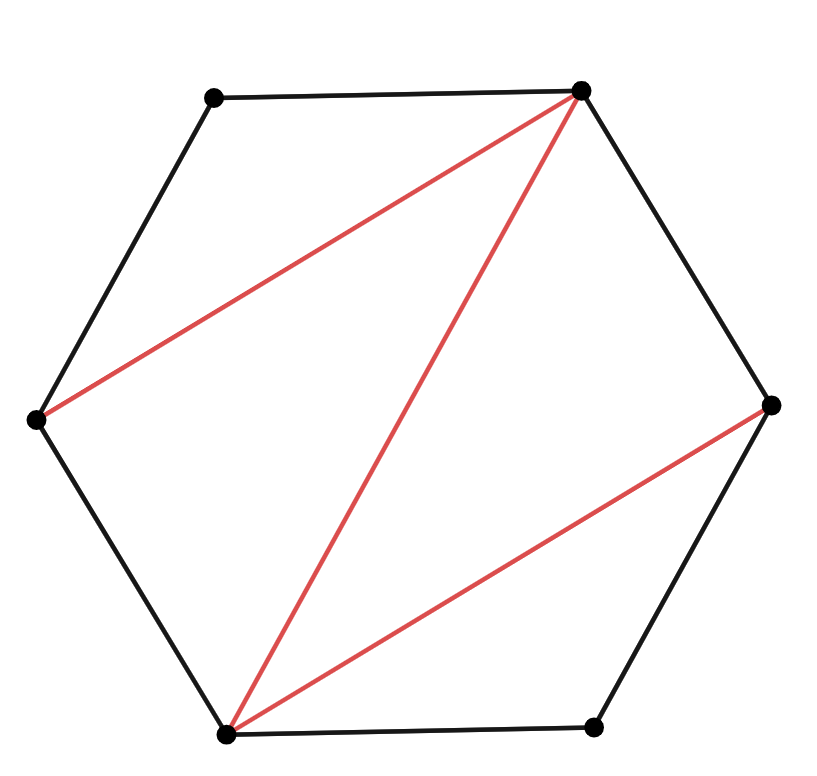
\includegraphics[scale=0.15]{images/grafos_poligonos_poliedros/triang_b_2.png}
		}
	\end{figure}
	
	\begin{figure}[H]
		\centering
		\subfloat[]{
			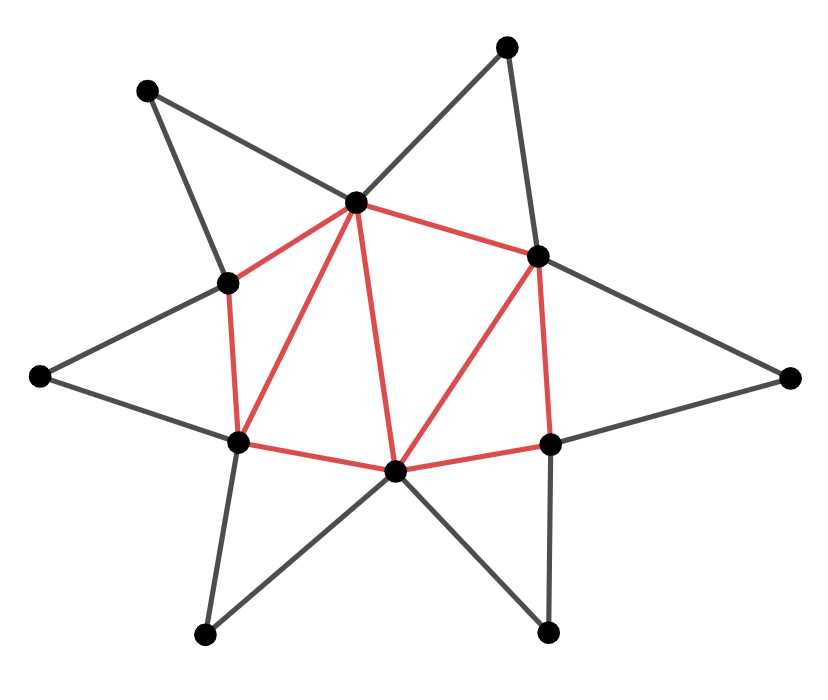
\includegraphics[scale=0.15]{images/grafos_poligonos_poliedros/triang_c_1.png}
			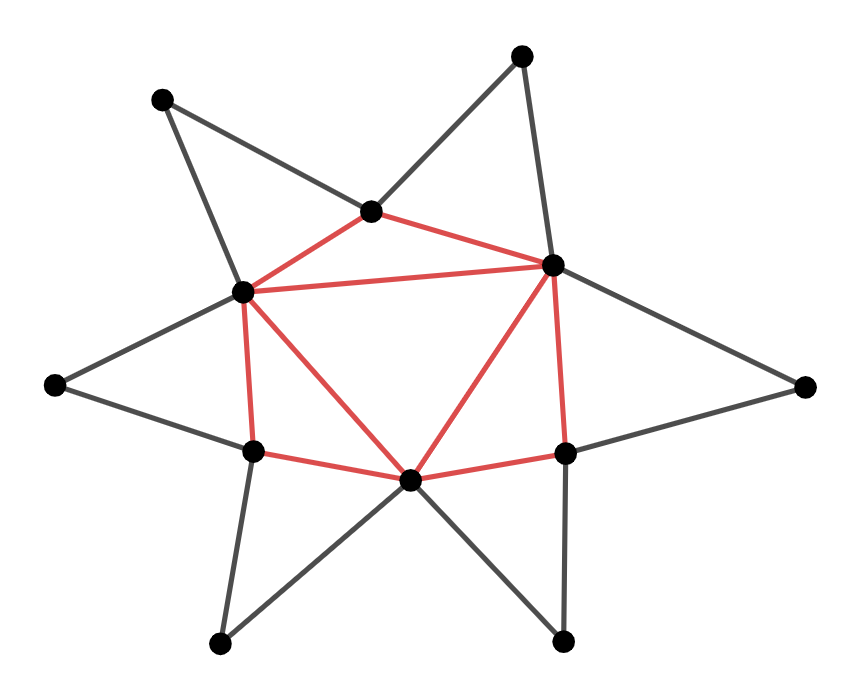
\includegraphics[scale=0.15]{images/grafos_poligonos_poliedros/triang_c_2.png}
		}
	\end{figure}
	
	
	\begin{figure}[H]
		\centering
		\subfloat[]{
			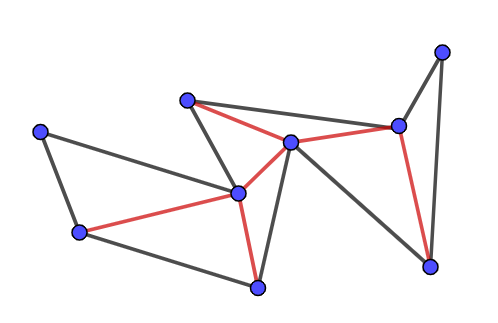
\includegraphics[scale=0.5]{images/grafos_poligonos_poliedros/triang_d_1.png}
			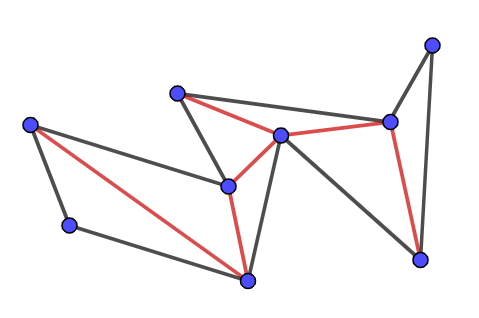
\includegraphics[scale=0.5]{images/grafos_poligonos_poliedros/triang_d_2.png}
		}
	\end{figure}
	
	
	
	\item Para todo $n$ encuentra un polígono con una única triangulación.
	
	Para que la triangulación sea única, el polígono ha de ser como los que mostramos en la imagen inferior (hasta $n=10$).
	
	\begin{figure}[H]
		\centering
		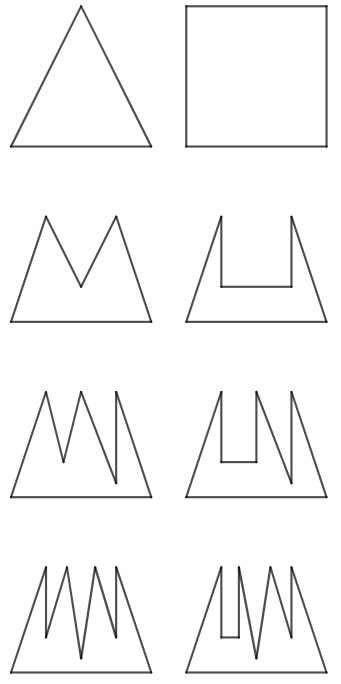
\includegraphics[scale=0.4]{images/grafos_poligonos_poliedros/triang_unica.png}
	\end{figure}
	
	Para los $n$ impares, debemos ``aislar'' los vértices como si en grupos con forma similar a $n=3$ y $n=5$ (lo podemos ver en el caso $n=9$) y de la misma manera con los $n$ pares utilizando los mismos valores que para el caso impar junto a $n=6$ (lo vemos en el caso $n=10$).
	
	
	
	
\end{enumerate}


\newpage
\begin{thebibliography}{X}

\bibitem{1} \textsc{Apuntes de Clase}

\end{thebibliography}


\end{document}

